\documentclass[letterpaper, 11pt, twocolumn]{article}
\usepackage[margin=1in]{geometry}
\setlength{\columnsep}{0.75cm}

\usepackage{fixltx2e}
\usepackage{tikz}
\usetikzlibrary{calc}
\usepackage{algorithm2e}
\usepackage{multirow}
\usepackage{graphicx}
\usepackage{amsmath}
\usepackage{cite}
\usepackage{framed, color}
\usepackage{color, soul}
\definecolor{shadecolor}{rgb}{.93,.93,.93}
\definecolor{blu}{rgb}{0,0,1}
\newcommand{\td}[1]{{\color{blu}\hl{TODO: #1}}}
\newcommand{\vwm}{$V_{w,n,k}$}
\newcommand{\wm}{$W_{w,n,k}$}
\usepackage{amssymb}
\usepackage{mathrsfs}
\usepackage{gensymb}

\title{Climate control for performant HPUs}
\author{}
 
\parindent0pt \parskip8pt
\begin{document}
\maketitle

\section*{Abstract}
\textbf{}
\section*{Introduction}
There are still many tasks for which humans outperform computers
These tend to be tasks that rely on a large repertoire of prior knowledge,
the excercise of common sense judgment, certain visual tasks, and 
tasks that require spontaneous hypothesis generation.

With the emergence of microtask platforms like Amazon Mechanical Turk (AMT),
comes the hope of building compute in which human intelligence can be accessed
on-demand.  This leads to an analogy of the human to the CPU, wherein we think
of human processing units.

A major challenge in building systems that deliver on this vision is the 
natual variability obtained in HPU output.  In some tasks, this variability
is desireable.  For example, in an image labelling task, the natural 
variability in
HPU output leads to greater coverage of the semantic space occupied by an 
image.  In other cases this variability can be problematic, such as in a 
transcription task, where there is only one corect output, and any variability
is only noise.

Whether desired or not, to build up efficient systems from HPUs, one must 
understand the natural variance quantitatively, and understand the factors that
influence it.

Here we model the variance between HPUs as comming from two sources.  The first
is a persistent, or intrinsic variability.  We imagine that this to encompass  
temperamental predispositions, life history, and developmental stage of the 
individual.  While
it may change over the course of a person's lifetime, in the view of the 
computational architect, it is essentially constant.

The seccond is a short-term variability, which arises from the fact that 
peoples immediate state is a function of recent events.  This would include
such things as an HPU becomming more efficient at a task once it has completed
a few tasks of the same type.  It would also include such things as the 
potentially detrimental effects of a noisy environment.

In this view, one can imagine HPUs being different in their specifications,
and also exhibiting hysteresis, whereby their output at some time $t$ is a
function of their inputs at time $t$, $t-1$, and so on.

In psychology, the act of producing these short-lived states that effect a
person's performance during a task is called \textit{priming}.  We will adopt
this term throughout the present work.


\section*{Prior Work}
Priming itself can be broken into many types, and many studies exist exploring
the effects of overt priming on the performance of HPUs. Priming may arise
due to how the task is framed.  This includes such things as the stated
purpose of the task, and the identity of the requester the task.

In \cite{chandler2013breaking}, the researchers investigate the effects of 
framing task either in a meaningful or meaningless way.  Compared to a 
zero-context control treatment, workers increase their output (for less pay),
when they are told that they are helping identify cancer, but there is no
change in quality.  When workers are told that their submissions will be 
discarded, there is no change in the amount of work done, but the quality 
declines.

Another source of priming can be due to what might be called 
\textit{sidestream information}: information that is presented to the 
individual but which is not actually salient to the task.

Other researchers have studied how having peer's responses available to 
the task could influence the worker.

In the present work, we focus on a more subtle source of priming, which arises
simply from the worker's performance in earlier stages of the task. 

We compare this to priming arising from framing the task by disclosing a 
(fictitious) funding agency that is paying for the study in which they are 
participating.

\section*{Framework}
At this point we have surveyed some of the conceptual framework traditionally
used to discuss priming in the context of psychology.  Having the origin that
they do, these frameworks are suited to describing the internal mechanisms of
the mind from which they arise.  For our purposes here, we are interested 
primarily in the \textit{effects} of priming, and so it makes sense to 
adopt a position conducive to those ends.  Since our interest in priming 
arises from a desire to construct computing systems from HPUs, we shall
propose a well-defined algorithmic definition for priming.

We must first remark that it does not make sense to speak of an un-primed 
state.  A person can be no more un-primed than a ship at sea can have no 
bearing.  Next, we propose that priming should generally be regarded as a
property of a population of HPUs, rather than as the state of a single HPU.
This is rather like the notion of temperature in thermodynamics.  Although
it does make sense to speak of the kinetic energy of a single molecule, 
Temperature is a statement about the distribution of kinetic energies in a
population of molecules.  The definition of priming which we presently submit
will also be defined in terms of populations.

Two populations, \textsc{j} and \textsc{k} are said to be 
\textit{differently primed} with respect to a task $\mathcal{T}$ if there 
exists a polynomial-time algorithm $\mathcal{A}$ that can distinguish 
(classify) members of \textsc{j} and \textsc{k} with accuracy $\theta$, when 
$\mathcal{A}$ is provided the labelled work-products of HPUs from \textsc{j} 
and \textsc{k} tasked with $\mathcal{T}$.
When $\mathcal{A}$ exists, we say that \textsc{j} and \textsc{k} deviate by 
$\theta$ in priming.

The above definition is simply intended to provide a well-defined definition
of what priming \textit{is}.  Naturally, it says nothing about the consequences
of priming.  The significance of the priming of a given population will
depend both on the nature of $\mathcal{T}$ and on the intended purpose of 
the work products derived from HPUs performing $\mathcal{T}$.


\section*{Methods}

\textbf{Task set-up.}
We paid 900 AMT workers to perform an image-labelling task.  A task consisted 
of labelling 10 images, with 5 labels each.  The first 5 images were varied 
depending on the priming treatment, while the last 5 images were the same 
accross all treatments.  Ordering of the images was kept constant.

Workers were randomly assigned to one of 6 treatments.  The treatments differed
from one another along two dimensions. The first dimension consisted of 
varying the first 5 images shown to the worker.  This was used to test the
effects of \textit{in-task} priming.

The second dimension concerned disclosure of a (fictitious) organization,
purportedly funding work as part of a research study.  Depending on the 
treatment, one of two funding agencies was presented, or no indication was 
made.

Tasks were presented to workers as a series of panels or flash cards.  The
first panel provided brief instructions, and was identical for all treatments.
Workers could see this panel when previewing the task, but could not advance.
Depending on the treatment, the worker was either shown a second pannel 
stating the name of 
one of two fictitious organizations funding the work, or this panel was 
skipped.  The next five pannels each consisting of a priming sub-tasks, 
wherein the worker was asked to submit five descriptive labels.  The images
used during the priming sub-task depended on the treatment.  The last 5 pannels
consisted of testing subtasks, wherein, as for the priming sub-tasks, workers
were asked to submit 5 descriptive labels.

\textbf{Choice of images.}
The 5 test images, were chosen with two ideals in mind.  
First, we chose images that we judged would generate a diverse vocabulary of 
labels, such that the effects of priming could be detected.  In other words,
sparse images with a single object in the foreground were not considered good 
candidates, since they would be less likely to elicit labels that varied from 
one worker and one priming treatment to the next.

Second, we chose images which would produce labels belonging to two broad
concepts, which would serve as the targets of our priming: food and culture.  
This created the opportunity to attempt to prime workers in a way that would
bias them toward emitting food-related or culture-related labels.

Under these considerations, we chose the images shown in 
Fig.~\ref{fig:testImages}.  Each of these images has food as its main focus,
but also has a strong and specific cultural reference due to the unique, 
iconic character of the food and the artifacts depicted.

To investigate in-task priming, we chose a set of images that highly
recognizeable cultural settings and no food, and another set that contained
separated food ingredients, without any overt cultural content.  The third
set of images was chosen to be very much like the test images, showing prepared
meals, and though prepared food is inseperable from culture, these images
were chosen based on being culturally more muted or ambiguous. 

\textbf{Label ontology.}
In order to provide a deeper analysis, we built an ontology
of the corpus of all labels applied to the first test image.  The ontology
was built as a directed acyclic graph starting 

\section*{Results and discussion}

\begin{figure*}
	\begin{center}
		\includegraphics[scale=0.55]{../figs/f1scores.pdf}
		\caption{caption here}
		\label{fig:classifier}
	\end{center}
\end{figure*}

\textbf{Priming affects HPU output.}
Before looking for differences in the content of labels provided by workers
from different treatments, we first demonstrate that the treatments are
distringuishable in an algorithmic sense.

Using a naive bayes classifier, we are able to distinguish with high precision
and specificity between workers from the \textsc{ambg} treatment and any of
the other 5 treatments.  Fig~\ref{fig:classifier}A shows F1-score for a
naive bayes classifier when distinguishing between the \textsc{ambg} and 
the other treatments. The classifier achieves high precision and specificity
in task.  Figure~\ref{fig:classifier}B shows the F1-score for binary
classification between the $\textsc{cult}_{img}$ and the other treatments, 
while \ref{fig:classifier}C shows that for $\textsc{ingr}_{img}$ and the other
treatments.  

Not surprisingly, pairs of treatments in which one primes for culture, and the
other primes for ingredients are easily distinguished.  However, it is quite
surprising that high accuracy is achieved when classifying treatments within 
the same valence (e.g. cultural).  This is especially true in such cases as
the classification of  $\textsc{cult}_{img}$ and $\textsc{cult}_{fund,img}$
($\text{F}_1 = 0.863$), where both treatments also share the priming images in 
common.

We find it remarkable that, using only the labels that workers provide, it is
possible to infer with good accuracy (at least when given a choice between 
two posibilities)  the treatment to which the worker was 
subjected.


\begin{figure}
	\includegraphics[scale=0.65]{../figs/valenceComparison.pdf}
	\caption{caption here}
	\label{fig:valence}
\end{figure}


\textbf{Priming orients HPU focus.}
Having established that each treatment does in fact consist of distinguishable 
populations of the HPUs, we next look at the content of labels.  Two of the
root labels in our ontology, \texttt{food} and \texttt{cultural}, map naturally
onto the two concepts that laid behind the design of our priming treatments.
A natural and straightforward expectation is that HPUs from treatments 
$\textsc{cult}_x$ should emit more labels that are ontological descendents of
\texttt{cultural}, while those from the $\textsc{ingr}_x$ treatments should
emit more labels under $\textsc{food}$.

In Fig.~\ref{fig:valence}, we exhibit the percentage of labels having a 
cultural valence (i.e. descending from \texttt{cultural} in the ontology), and 
the percentage having a food valence. Before making comparisons using this
information, we remark that there is no reason to expect a balance in the 
number of words having cultural or food valence overall.  The $\textsc{ambg}$
treatment, which was designed to promote neither valence, exhibits a
significant fraction of words from both the food and cultural valence, while
significantly favoring the former.  

Both $\textsc{cult}_{img}$ and $\textsc{cult}_{fund,img}$ show a significant
excess of culturally-oriented labels and fewer food-orientel labels.  
Furthermore, HPUs in these treatments emit more culturally-oriented labels 
even while emitting fewer labes that are simultaneously oriented toward 
cultural and food (light bars in Fig.~\ref{fig:valence}).
The deviation of these treatments from
the others is well beyond the 95\% confidence interval.

Interestingly, the $\textsc{cult}_{fund}$ treatment did not have this effect.
Although we have demonstrated that $\textsc{cult}_{fund}$ is differently
primed from \textsc{ambg} using a naive bayes classifier, in respect of 
overal fraction of food- and culturally-oriented labels, no distinction 
is to be made.

In the case of $\textsc{ingr}_x$ treatments one expects to see an 
enrichment of food-oriented labels. There is perhaps some evidence for this
$\textsc{ingr}_{fund}$ and $\textsc{ingr}_{fund,img}$, but we cannat make any
assertion with confidence.


\begin{figure*}
	\includegraphics[scale=0.65]{../figs/specificity2.pdf}
	\caption{caption here}
	\label{fig:specificity}
\end{figure*}

\textbf{Priming affects attention to detail.}
We next look at how alternately treated HPUs differ in their tendency to use
more specific or more general labels. We use the ontology of labels emitted
on the first test image to unambiguously establish a partial ordering of 
label-specificity.  If one label $\ell_1$ is within the ancestry of another
$\ell_2$, we say that $\ell_1$ is more general than $\ell_2$, otherwise they
are not comparable.  Thus, the label \texttt{naan} is more 
specific than both \texttt{bread} and \texttt{indian}, while uncomparable to
\texttt{statue}.

Label-specificity only generates a partial ordering---at least in our 
experimental design.  A consequence of this is that it is not possible to
assign an overall specificity score to a set of labels.  We submit that this
reflects the underlying complexity of natural language semantics.  While
we admit that there may be many ways to generate full orderings based on some
notion of label specificity, we believe that this would inappropriately 
collapse qualitative differences between labels, leading to results that are
difficult to interpret.

In Fig.~\ref{fig:specificity}, We show pairwise specificity comparisons 
between various pairs of treatments.  Figure~\ref{fig:specificity}A shows
the comparison of \textsc{ambg} with all other treatments.  Both treatments
primed with cultural images ($\textsc{cult}_{img}$ and 
$\textsc{cult}_{fund, img}$) exhibit an excess of more general words compared
to \textsc{ambg}.  Meanwhile, $\textsc{ingr}_{fund}$ emitted an excess of 
more specific words.

We can seek to explain these observations by restricting the comparison to
labels of a specific orientation (e.g. food or cultural).  When we perform
the same comparisons but restricting to food-oriented labels, as shown in 
Fig.~\ref{fig:specificity}G, we see some of the same tendencies as in A.
However, when restricting to culturally-oriented labels 
(Fig~\ref{fig:specificity}D) there are no significant comparative deviations 
in specificity to speak of.

A first conclusion that we can draw from this is that there is a significant
loss of specificity in labels emitted by treatments having non-ambiguous 
priming images.  In Fig.~\ref{fig:specificity}G, only $\textsc{cult}_{fund}$
and $\textsc{ingr}_{fund}$ show no significant deviation.  

- through negative priming workers stop responding to generic features of images of prepared meals, which happens in the ambiguous case.

- On the other hand, workers presented with either the cultural or ingredients images are initially struck by the gross differences, which draws generic 
labels, especially with respect to food for which generic labels in ambiguous treatment had been suppressed through negative priming.

- it seems, at first, inconsistent that $\textsc{cult}_{img}$ and 
$\textsc{cult}_{fund,img}$ would at once enrich the fraction of 
culturally-oriented words, but produce no change in the specificity of 
culturally oriented words.  First of all, there is no logical incompatibility
with producing a greater number of cultural terms, yet which are generic 
in nature.  If we follow the hypothesis that focus (or orientation) is directed
by positive priming (perhaps through the subconscious or conscious inference
of reqeuster intent), while focusing on nuances comes from the inhibition
of gross features through negative priming, then this combination of observations makes sense.  Having seen many cultural images, HPUs in 
$\textsc{cult}_{img}$ and $\textsc{cult}_{fund,img}$ are primed to emit 
cultural labels, however, since the diversity of images is high compared to
other treatments on reaching the test images, there no opportunity for 
focussing in to finer detail through the mechanism of negative priming.

\begin{figure}
	\includegraphics[scale=0.4]{../figs/longitude0.pdf}
	\caption{caption here}
	\label{fig:longitude}
\end{figure}


One interesting test of this hypothesis arises in 
% Graphics commented out because they make compiling take long!  
% Uncomment when desired!
\begin{figure*}
%	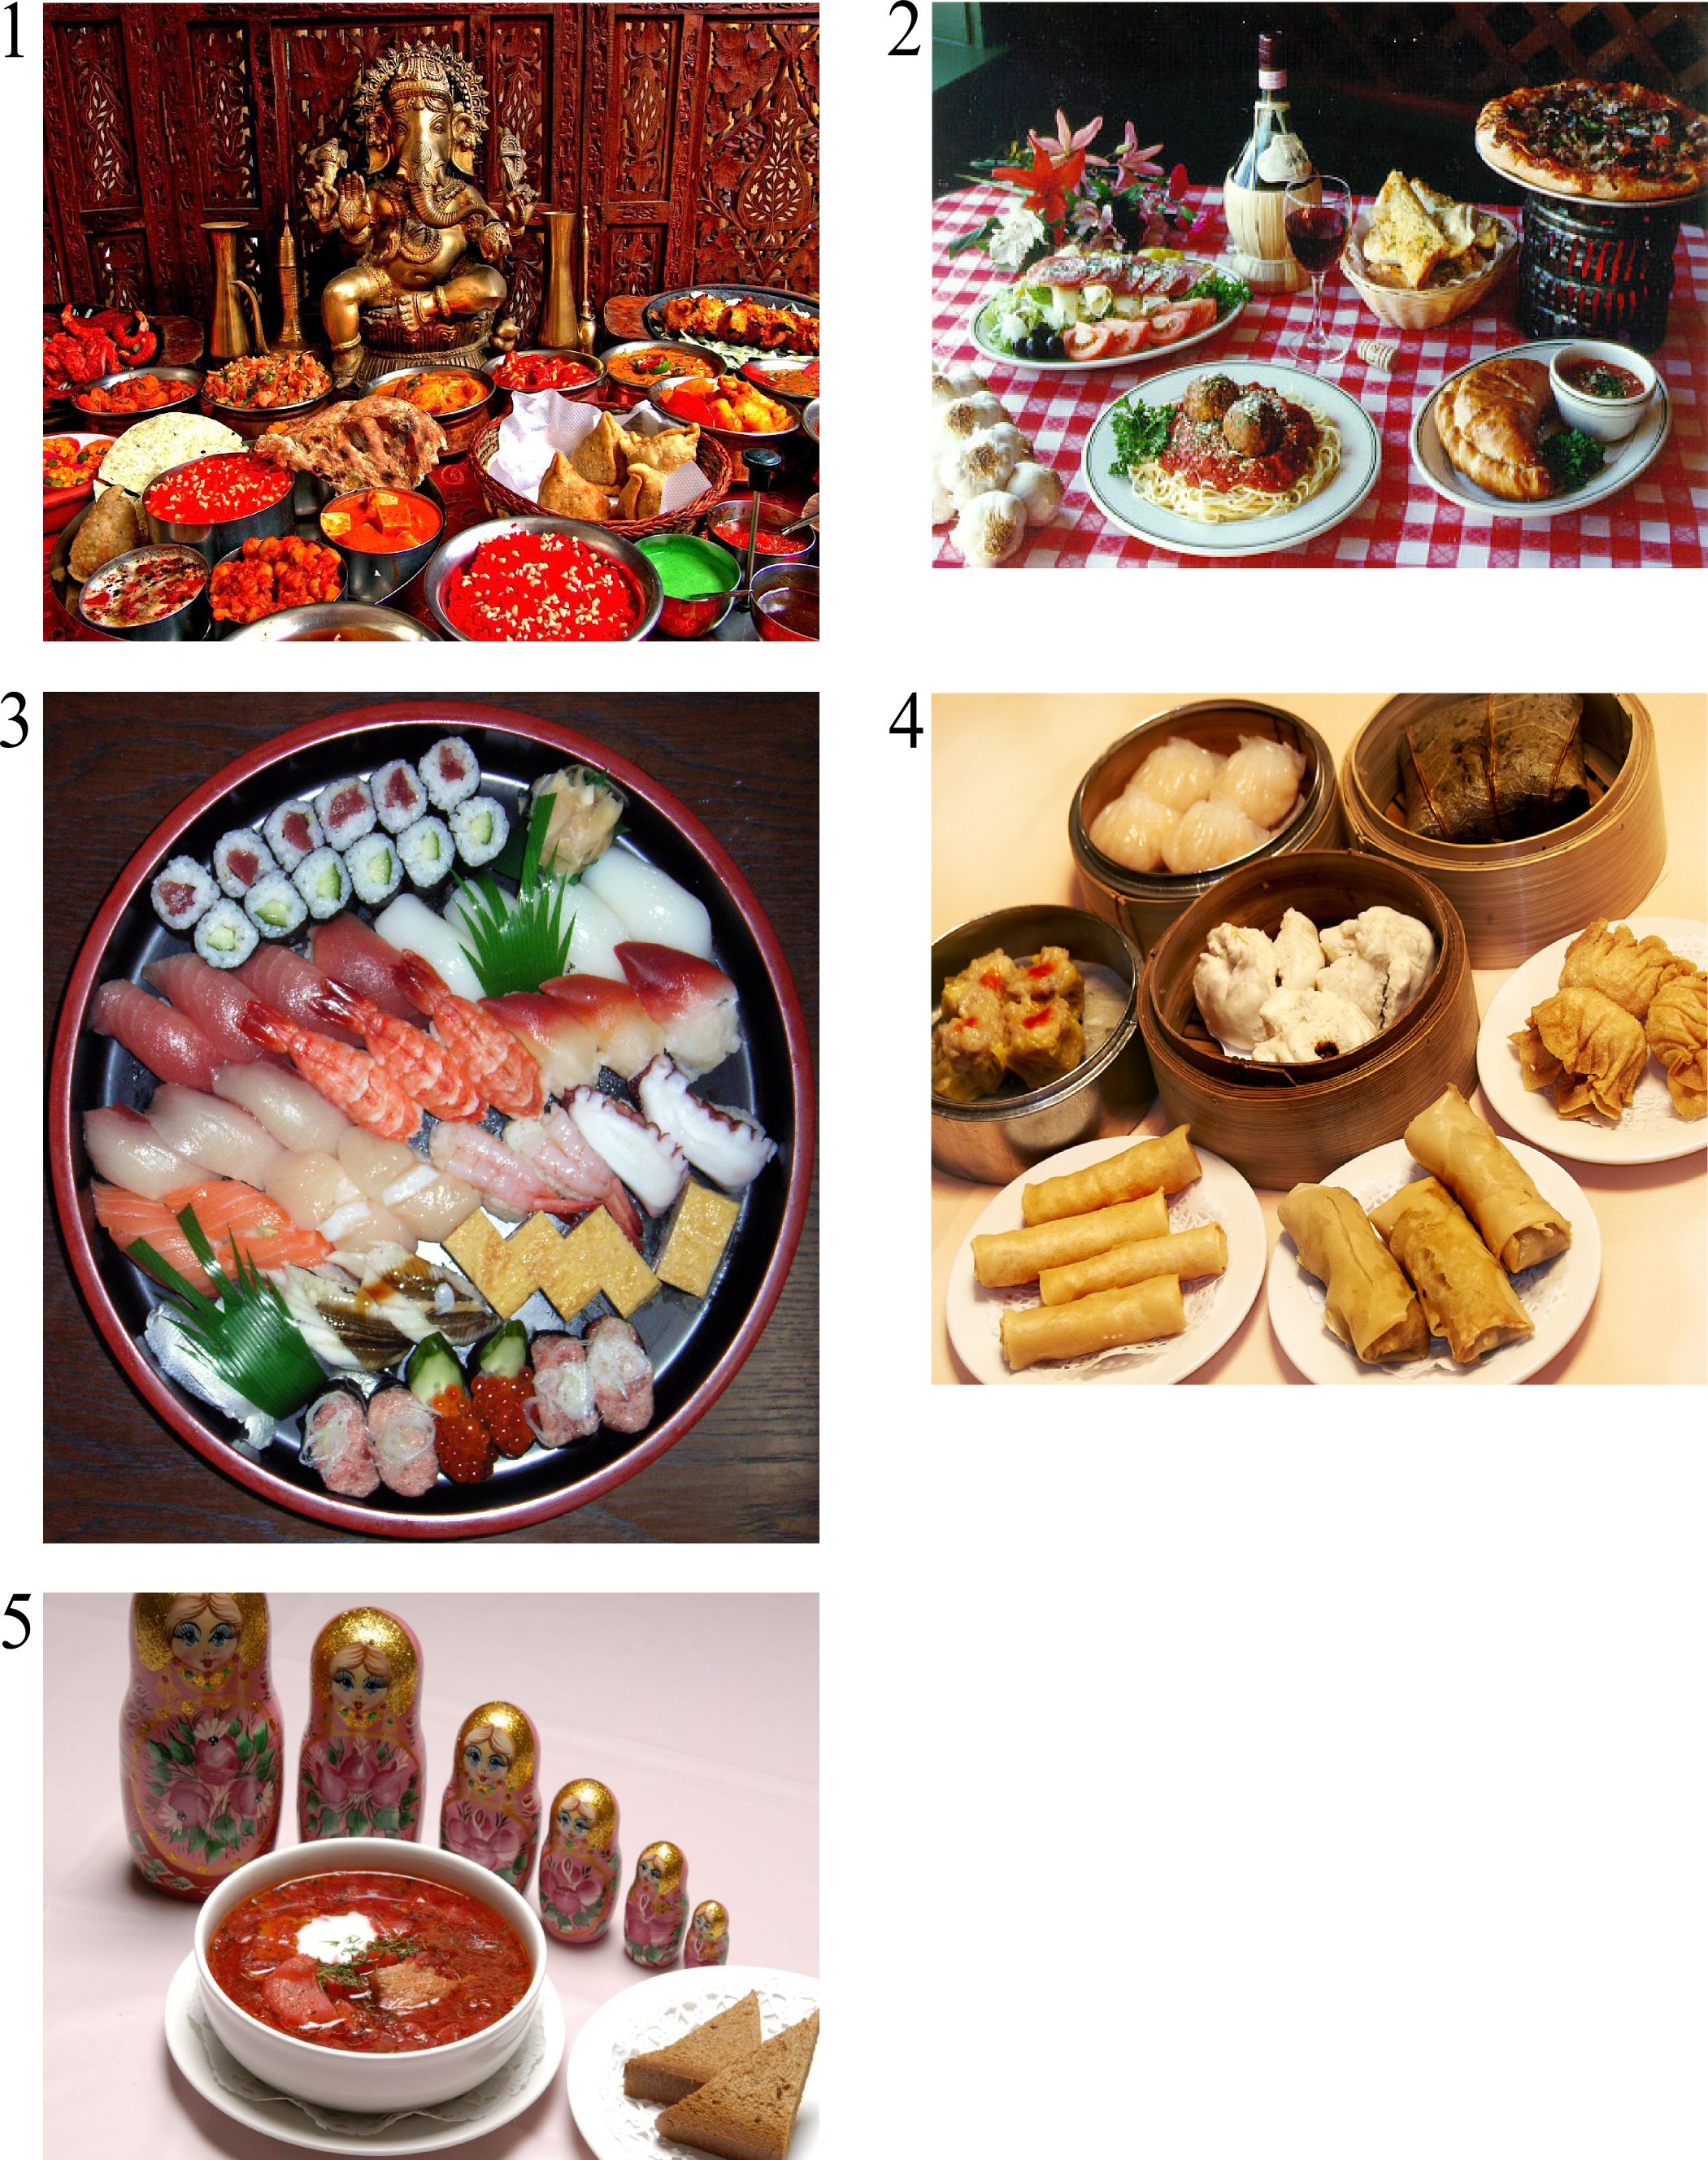
\includegraphics[scale=1.00]{../figs/testImages.png}
	\caption{caption here}
	\label{fig:testImages}
\end{figure*}

\begin{figure*}
%	\includegraphics[scale=1.00]{../figs/ambiguous.png}
	\caption{caption here}
	\label{fig:ambiguous}
\end{figure*}

\begin{figure*}
%	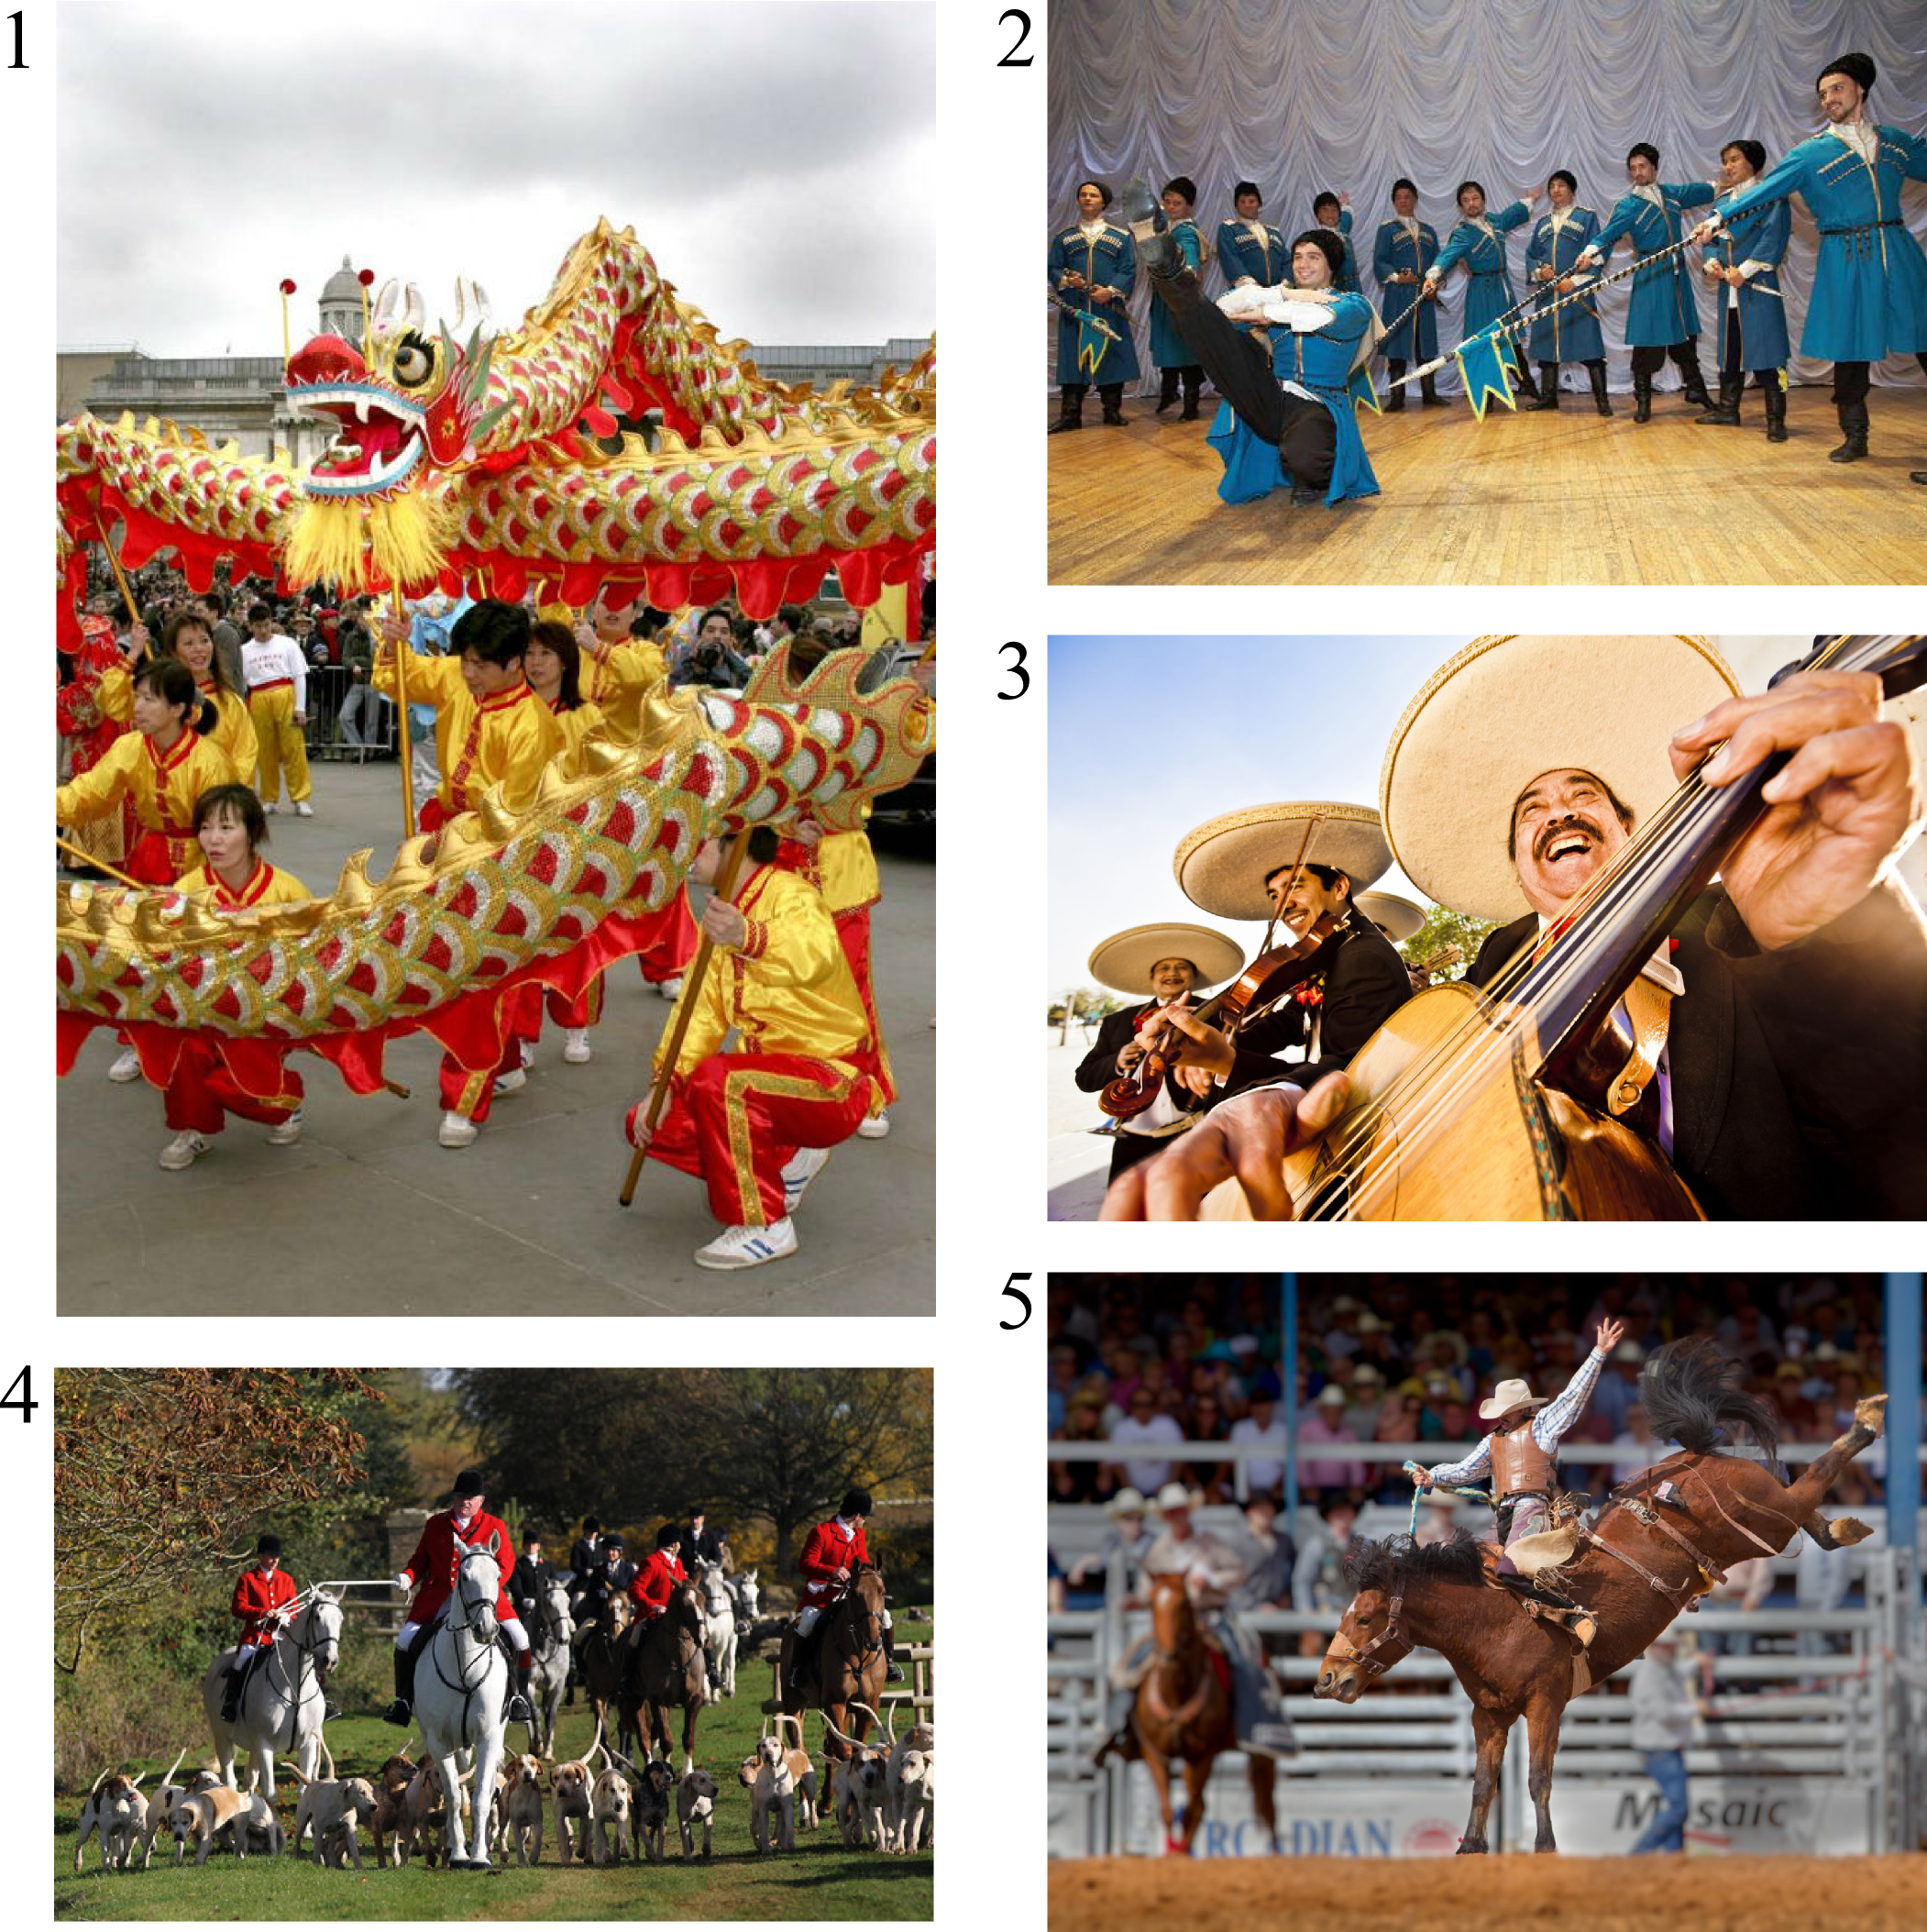
\includegraphics[scale=1.00]{../figs/cultural.png}
	\caption{caption here}
	\label{fig:cultural}
\end{figure*}

\begin{figure*}
%	\includegraphics[scale=1.00]{../figs/ingredients.png}
	\caption{caption here}
	\label{fig:ingredients}
\end{figure*}

\bibliographystyle{plain}
\bibliography{bab.bib}
\end{document}
